\documentclass[10pt,a4paper]{article}
\usepackage[utf8]{inputenc}
\usepackage[margin=0.75in]{geometry}
\usepackage{amsmath}
\usepackage{amsfonts}
\usepackage{amssymb}
\usepackage{graphicx}
\usepackage{hyperref}
\usepackage{dirtree}
\author{Chris Mamon}
\title{Angiography + OCT Reconstruction in Python: Setting things up}
\date{}
\begin{document}
	\maketitle
	\section{Package/Environment Managers and Editors}
		Before we dive into the reconstruction we need to set up a python environment and editor. The package and virtual environment manager we have chosen is \textbf{Miniconda} and the editor is \textbf{Visual Studio Code} (VSC).
		
		\href{https://docs.conda.io/en/latest/miniconda.html}{Miniconda} is a free minimal installer for \href{https://www.anaconda.com/distribution/}{conda}. We will use it to manage python packages and environments. If you are unfamiliar with these two terms:
		\begin{itemize}
			\item \href{https://realpython.com/python-modules-packages/#reloading-a-module}{Packages}: Are hierarchical structures 	containing python programs.	
			\item \href{https://www.geeksforgeeks.org/python-virtual-environment/}{Virtual Environments}: Isolate python dependencies from ones another, allowing developers to easily separate projects on the same device.
		\end{itemize}
		\begin{figure}[h]
			\centering
			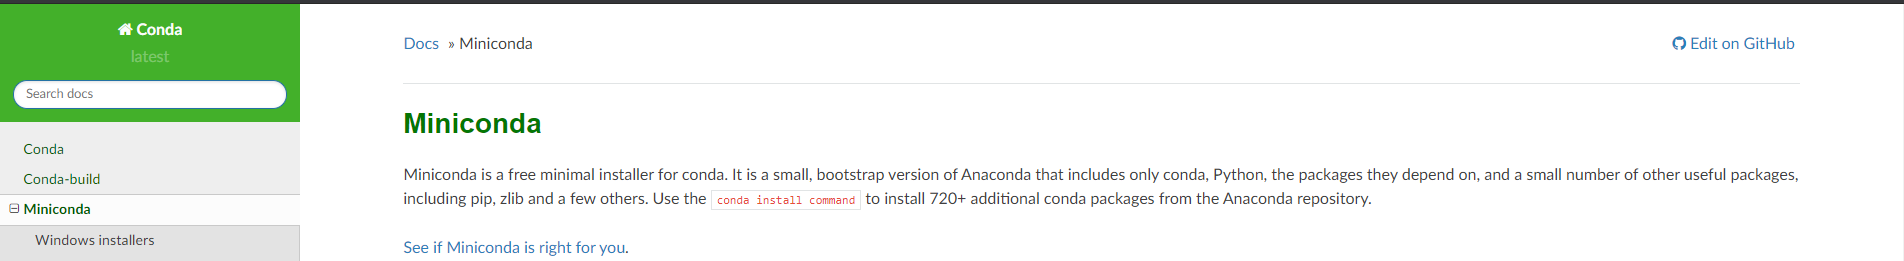
\includegraphics[scale=0.25]{figures/miniconda.PNG}
			\caption{Miniconda download and documentation page \url{https://docs.conda.io/en/latest/miniconda.html}}
		\end{figure}
		
		\href{https://code.visualstudio.com/}{Visual Studio Code} is a source-code editor developed by Microsoft for Windows, Linux and macOS. It includes support for debugging, embedded Git control and GitHub, syntax highlighting, intelligent code completion, snippets, and code refactoring. It is my personal editor of choice due to its light weight nature, high customizability and powerful debugging.
		\begin{figure}[h]
			\centering
			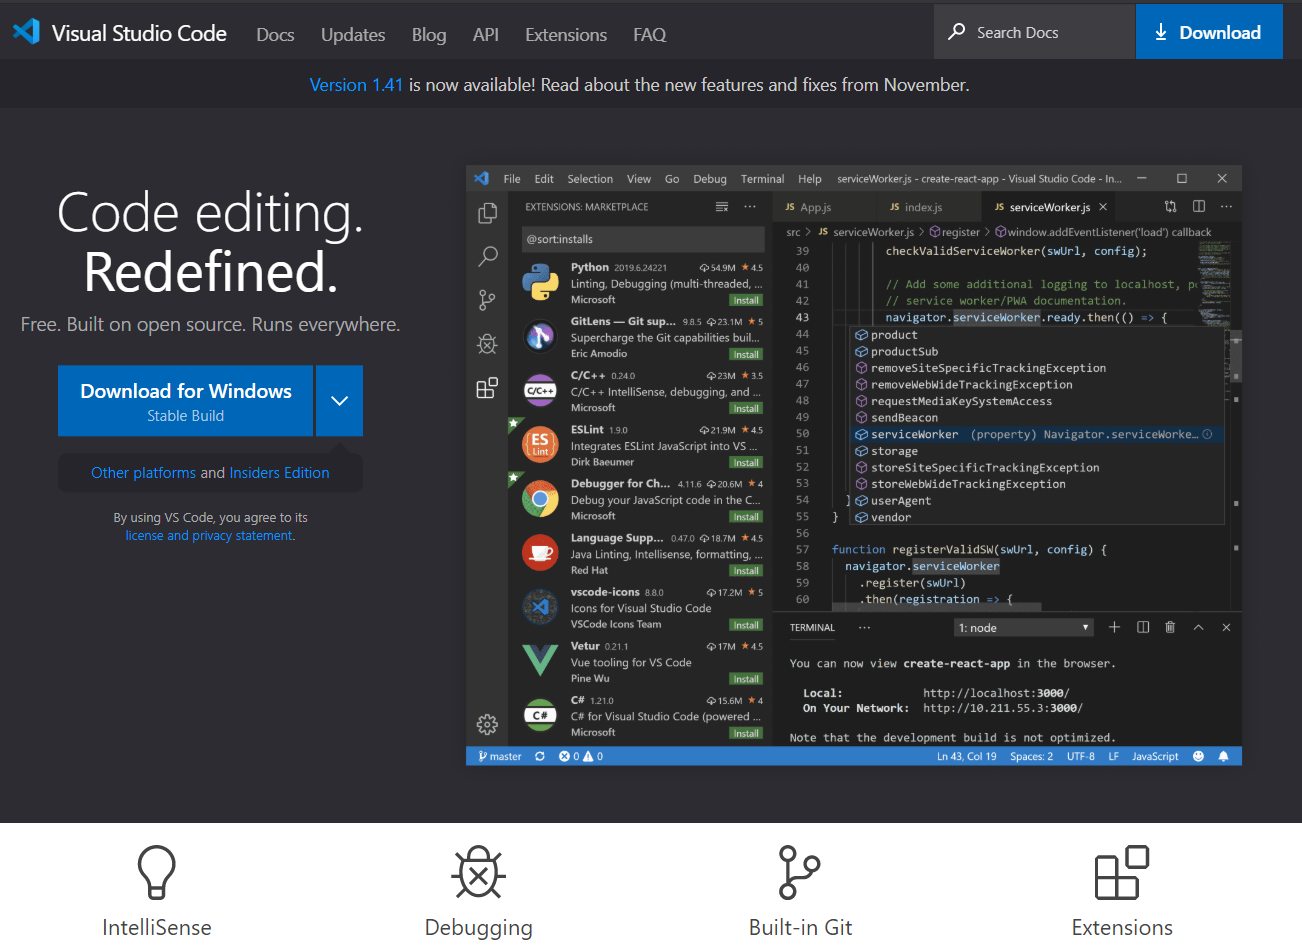
\includegraphics[scale=0.25]{figures/vsc_page.PNG}
			\caption{Visual studio code homepage \url{https://code.visualstudio.com/}}
		\end{figure}
	\section{Github}
		\href{https://github.com/}{Github} is a \href{https://git-scm.com/}{Git} repository hosting service. Git is a distributed version-control system for tracking changes in source code during software development. The \href{https://github.com/hj40/pymethods}{source code} for this project hosted in github and can be downloaded directly from \url{https://github.com/hj40/pymethods.git}.
	\section{Setting up a Miniconda Environment in Visual Studio Code}
		To use our miniconda extension in VSC we first need to install the \href{https://marketplace.visualstudio.com/items?itemName=ms-python.anaconda-extension-pack}{Anaconda Extension Pack}. This can be done directly through the VSC extensions tab, figure \ref{fig:VSCAnacondaExtension}
		\begin{figure}[h]
			\centering
			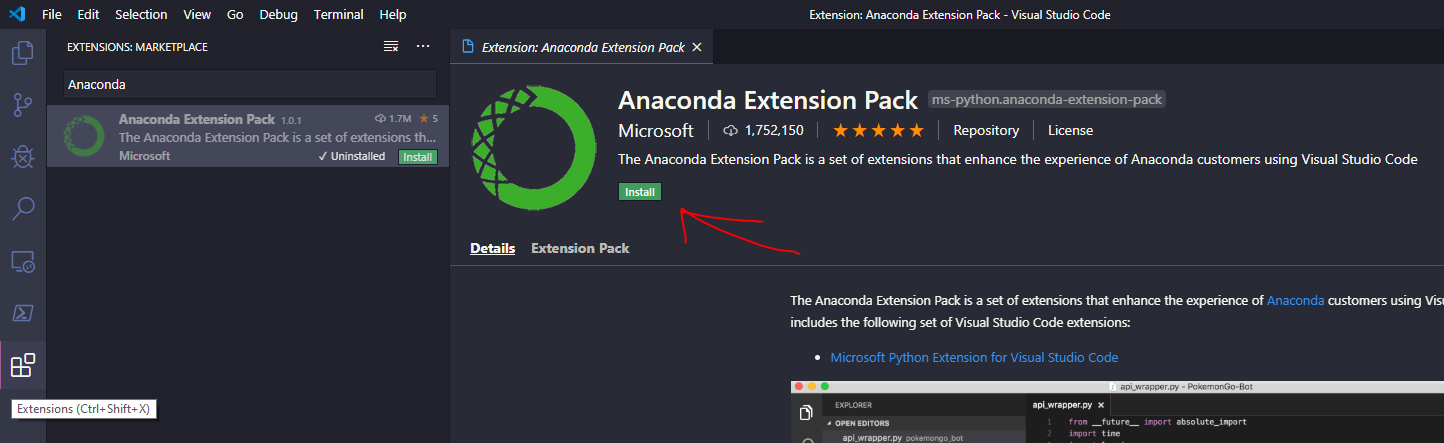
\includegraphics[scale=0.4]{{figures/AnacondaVSC.PNG}}
			\caption{VSC Extension market place press the green install button to install the Anaconda Extension Pack}
			\label{fig:VSCAnacondaExtension}
		\end{figure}
	
		Let us now open us a new integrated terminal in VSC.
		\begin{figure}[h]
			\centering
			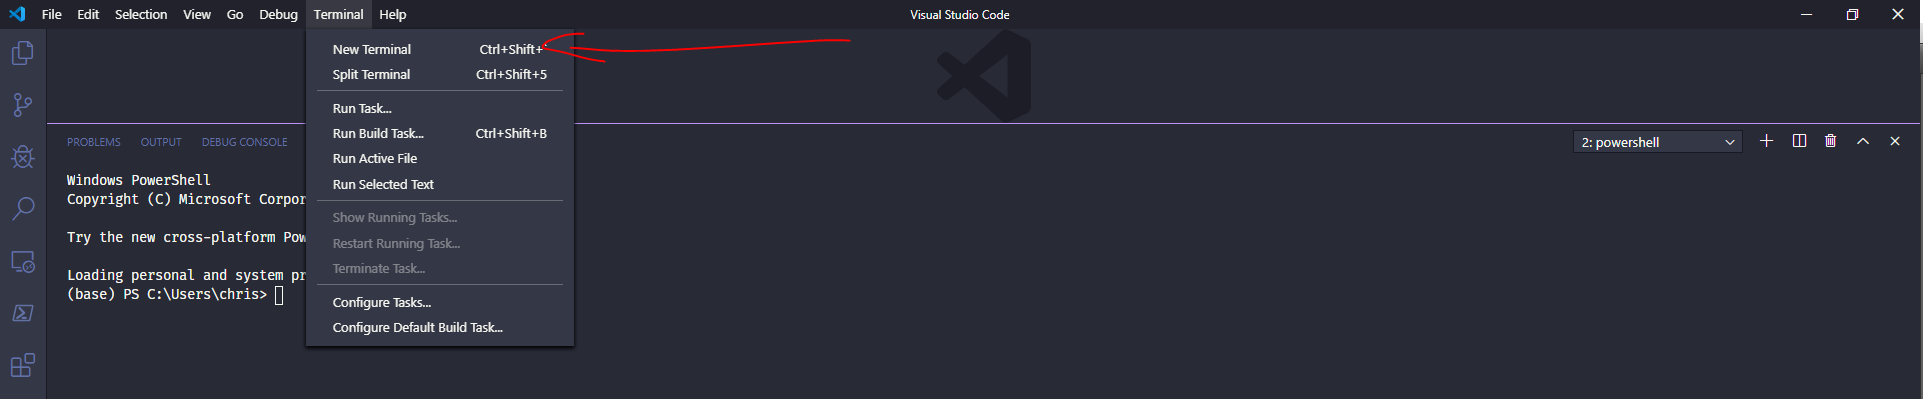
\includegraphics[scale=0.32]{figures/VSCTerminal.PNG}
			\caption{Opening a new terminal in VSC. The integrated terminal has popped up bellow. More information about the terminal can be found at \url{https://code.visualstudio.com/docs/editor/integrated-terminal}}
		\end{figure}
		
		From the terminal we can create and activate miniconda. If using powershell, i.e. using windows we must first call
		
		\begin{verbatim}
			conda init powershell
		\end{verbatim}
		
		To create a miniconda environment called \textit{myenv} we use the following command.
		
		\begin{verbatim}
			conda create --name myenv
		\end{verbatim}
		
		Once the environment is created we can activate it using ,
		\begin{verbatim}
			conda activate myenv
		\end{verbatim}
	\section{Environment Variable Definitions}
		Let us say we are developing on multiple packages and want to easily mingle them together. For example we have the following packages,
			\dirtree{%
				.1 /.
				.2 package A.
				.3 modules A.
				.2 package B.
				.3 modules B.
				.2 package C.
				.3 modules C.
			}
		We must include these in the \textit{PYTHONPATH} environment variable. Though this can be done within a terminal, the specified changes are transient. To make them persist we can modify our \textit{profile/rc} files. 
		\subsection{Windows Powershell}
			In windows \href{https://docs.microsoft.com/en-us/powershell/scripting/overview?view=powershell-7}{Powershell} this is managed from the \%PROFILE\% file. In VSC we can run,
			\begin{verbatim}
				code $PROFILE$
			\end{verbatim}
			This will open up the file within VSC, and we can add the following lines to the file,
			\begin{verbatim}
				$env:PYTHONPATH = "$env:PYTHONPATH;<path to package A>;<path to package B>;..."
			\end{verbatim}
		\subsection{Mac Bash}
			In MAC OSX \href{https://help.ubuntu.com/community/Beginners/BashScripting}{Bash} our profile is managed in the bash\_profile file located from within our \$USER directory. To open the file we can run,
			\begin{verbatim}
				code $USER/.bash_profile
			\end{verbatim}
			Now to extend out PYTHONPATH we add the following lines
			\begin{verbatim}
				export PYTHONPATH="${PYTHONPATH}:<path to package A>:<path to package B:..."
			\end{verbatim}
		Perform this for the repository downloaded from github
		
	\section{Setting up a folder in VSC}
		Now we can open up the package folder in VSC to the repository downloaded from github, figure \ref{fig:openFolder}. This allows us to view the directory tree structure in visual studio and apply \href{https://code.visualstudio.com/docs/python/linting}{linting} and \href{https://code.visualstudio.com/docs/python/debugging}{debugging tools}.
		\begin{figure}[h]
			\centering
			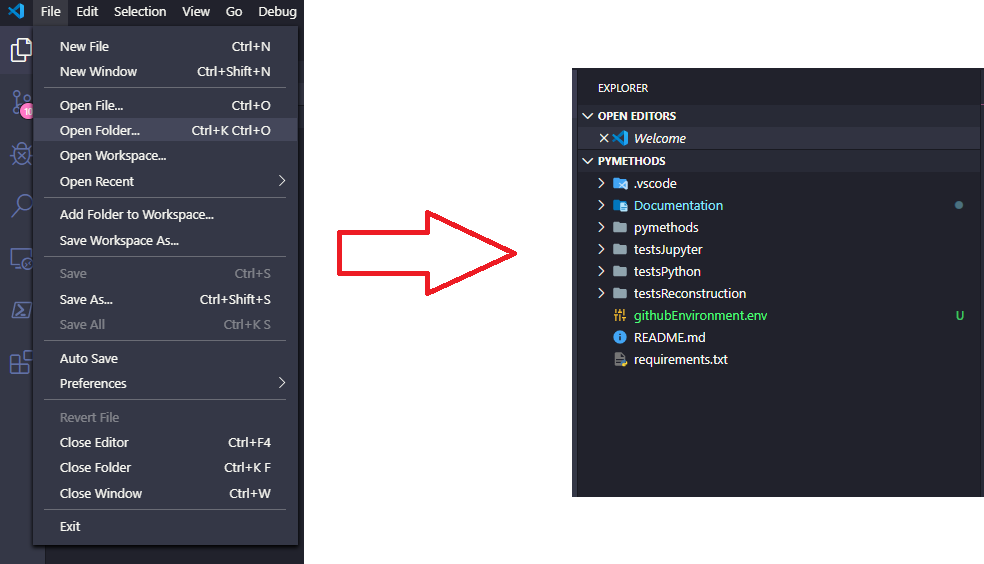
\includegraphics[scale=0.5]{figures/folder.PNG}
			\caption{Opening a folder in visual studio code}
			\label{fig:openFolder}
		\end{figure}
	
		Initially our conda environment is might not be selected. To select our desired python interpreter (i.e. environment) we can open a command panel with \verb|ctr+shift+p| and by searching for \verb|python interpreter|, \ref{fig:selectInterpreterCommandPanel}, we can view a list of our available python interpreters, figure \ref{fig:interactiveSelectInterpreter}.
		
		\begin{figure}[h]
			\centering
			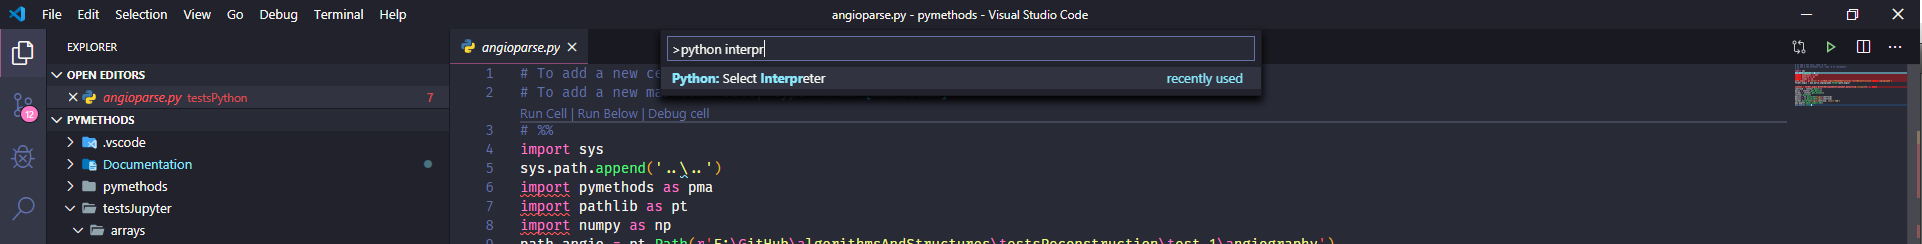
\includegraphics[scale=0.3]{figures/select_interporeter_A.PNG}
			\caption{Finding the select interpreter method from the command panel}
			\label{fig:selectInterpreterCommandPanel}
		\end{figure}
	
	 	we can also click the interpreter button at the bottom left of the screen \ref{fig:interactiveSelectInterpreter},

		\begin{figure}[h!]
			\centering
			\includegraphics[scale=0.25]{figures/select_interpreter_b.PNG}
			\caption{Interpreter selection after running select interpreter from the command panel. This panel can also be opened interactively by pressing the button circled in red}
			\label{fig:interactiveSelectInterpreter}
		\end{figure}
	
		\newpage
	\section{Installing Requirements}
		once the interpreter has been selected the python packages required for the Angiography + OCT Reconstruction package can be installed quickly via the \href{https://pypi.org/project/pip/}{pip} package installer. Run the following command from the terminal,
		\begin{verbatim}
			python -m pip install -r <path>/requirements.txt
		\end{verbatim}  
		
	
\end{document}